\subsection{Matrix Multiplication}

\begin{figure*}[t]
    \centering
    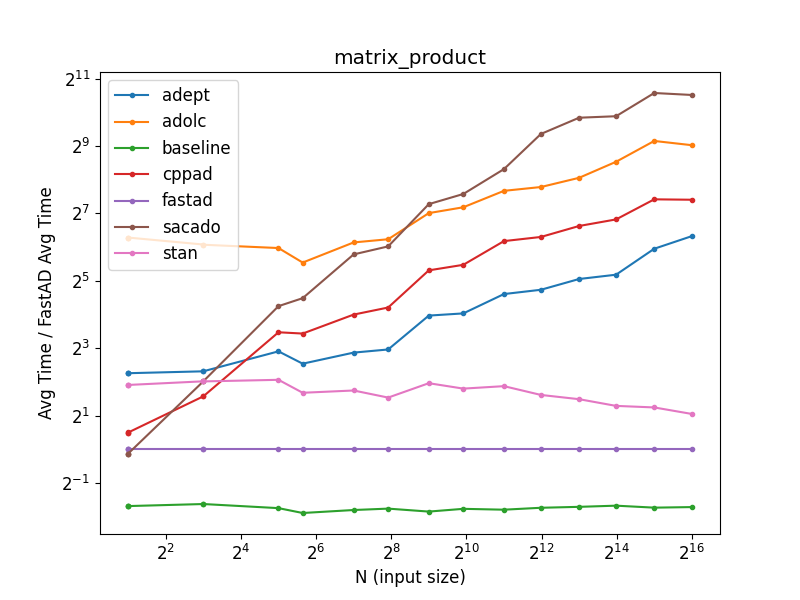
\includegraphics[width=\textwidth]{figs/matrix_product_fig.png}
    \caption{%
        Matrix multiplication benchmark of other libraries against FastAD 
        plotted relative to FastAD average time.
    }\label{fig:matrix_mult}
\end{figure*}

For this benchmark, all matrices are square matrices of the same size.
The functor fills the x vector by first resizing it to $2 \cdot K^2$,
where each matrix is $K\times K$.
In order to have a scalar target function,
we add another step of adding all of the entries of the matrix multiplication, i.e.
\[
    f(A, B) = \sum\limits_{i=1}^{K} \sum\limits_{j=1}^{K} {(A \cdot B)}_{ij}
\]
Hence, we could not benchmark with $N$ at exact powers of $ 2$,
however, the modified range of values for $N$ still shows a meaningful trend.
We also tested $N$ larger than $2^{14}$ since it was not enough to show any convergent behavior.
All libraries except Adept and Stan were excluded from this benchmark
because they did not provide suitable support for matrix multiplication
and the default overload using \verb|Eigen| API exceeded the time limit.
All tested libraries provided built-in functions to 
compute the matrix multiplication and sum the elements.
Fig.\ref{fig:matrix_mult} shows the benchmark results.

FastAD is still the fastest library for all values of $N$, 
but Stan performs much closer to FastAD than the previous examples.
Adept consistently performs worse compared to FastAD and Stan.
The trend stabilizes towards the end at around $N=2^{14}$ where 
Stan is about $ 2$ times slower.
For moderate sized $N \in [2^{8}, 2^{10}]$, Stan is about 3--4 times slower.

The comparison with the baseline shows that FastAD takes $ 3.14$ times longer.
Note that forward-evaluation requires one matrix multiplication between two $N\times N$ matrices,
and backward-evaluation also requires two matrix multiplications of the same order,
one for each adjoint:
\begin{align*}
    \frac{\partial f}{\partial A} 
    &= \frac{\partial f}{\partial (A\cdot B)} \cdot B^T \\
    \frac{\partial f}{\partial B} 
    &= A^T \cdot \frac{\partial f}{\partial (A\cdot B)}
\end{align*}
Hence, one gradient evaluation requires three matrix multiplications between two $N\times N$ matrices.
As a rough estimate, if we approximate a manually-written gradient computation to be
three times the baseline (one multiplication), FastAD time relative to this approximate manual gradient computation time
is $\frac{3.14}{3} = 1.0475$.
This shows then that FastAD only has about $ 4.75\%$ overhead 
from a manually-written code, which is extremely optimal.
